\newcommand{\Lepp}[1]{\mbox{Lepp}(#1)}
\theoremstyle{definition}
\newtheorem{definition}{Definición}[section]

\newtheorem{theorem}{Teorema}


\newtheorem{lemma}[theorem]{Lema}

\newcommand{\ttt}{\texttt}
\DeclarePairedDelimiter\ceil{\lceil}{\rceil}
\DeclarePairedDelimiter\floor{\lfloor}{\rfloor}
 
\chapter{Introducción}\label{chap:intro}
En el contexto la astronomía observacional, la medición continua de la magnitud de una fuente, como una estrella o una galaxia, permite la construcción de su curva de luz, que caracteriza la variación de la magnitud en función del tiempo. De esta curva de luz, es posible extraer características, o {\it features}, como su periodo y los parámetros de un ajuste sinusoidal, y usar estas características para clarificarla y hacer conclusiones sobre su naturaleza.%, como se ilustra en la figura \ref{fig:ebvsrrl}.
\begin{comment}
    
\begin{figure}[h]
    \centering
    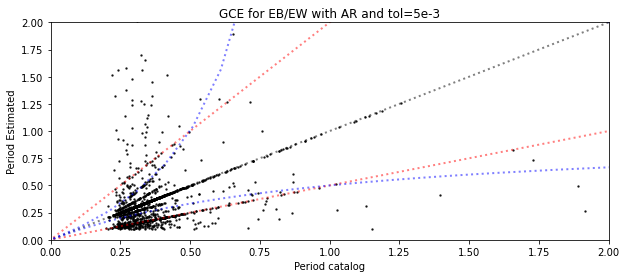
\includegraphics[width=0.8\textwidth]{placeholder.png}
    \caption{Curvas de luz de un sistema binario eclipsante (Figura superior), compuesto por dos estrellas que se eclipsan periódicamente, y una estrella RR Lyrae (Figura inferior), que pulsa gradualmente por un periodo determinado, tienen curvas de luz marcadamente diferentes y es posible diferenciarlas de esta manera.
}
    \label{fig:ebvsrrl}
\end{figure}
\end{comment}
El broker astronómico ALeRCE (Automatic Learning for Rapid Classification of Events) tiene el propósito de procesar el flujo de alertas de variabilidad astronómicas proveniente de telescopios de rastreo, calcular características de las curvas de luz asociadas a las alertas y usarlas para clasificar la fuente usando Machine Learning, y así permitirle a los astrónomos evaluar si vale la pena estudiar alguna de estas alertas y dedicarle valioso tiempo de observación. \cite{alerce-intro}

Una de las características más importantes de las curvas e luz es el periodos, que se calcula mediante un periodograma, que a cada frecuencia de prueba $\omega$ le asigna una medida de confianza $\Theta(\omega)$ cuyo valor determina que tan bien se ajusta cada frecuencia a la curva de luz al doblarla, lo cual consiste en definir la fase $\phi$, definida por $\phi(t) \equiv t/T + \floor{t/T}$ y graficar la magnitud en función de la fase.

El periodograma usado actualmente en ALeRCE es el {\it Multiharmonic Analysis of Variance} (MHAOV), que ajusta un sinusoide con un determinado número de armónicos a la curva doblada con una frecuencia $\omega$ y define como $\Theta(\omega)$ como un valor que define que tan bien se ajusta este sinusoide a la curva de luz. \cite{MHAOV}. Actualmente, MHAOV es un algoritmo que se ejecuta completamente en CPU, y es impreciso para ciertos situaciones que se describirán en las siguientes secciones.

\section{Motivación}\label{sec:motivacion}
El periodo de las curvas de luz una de sus propiedades más importantes ya que permite diferenciar entre objetos con curvas de luz similares pero distintos rangos de periodos y al estudiar la fuente en sí el periodo suele ser relevante para derivar propiedades físicas de las fuentes, como la distancia o su masa de las estrellas, además, el cálculo del periodo es actualmente una de las características mas computacionalmente costosas de calcular del sistema ALeRCE, y es por esto que es de gran importancia mejorar su precisión y eficiencia.

\begin{figure}[H]
    \centering
    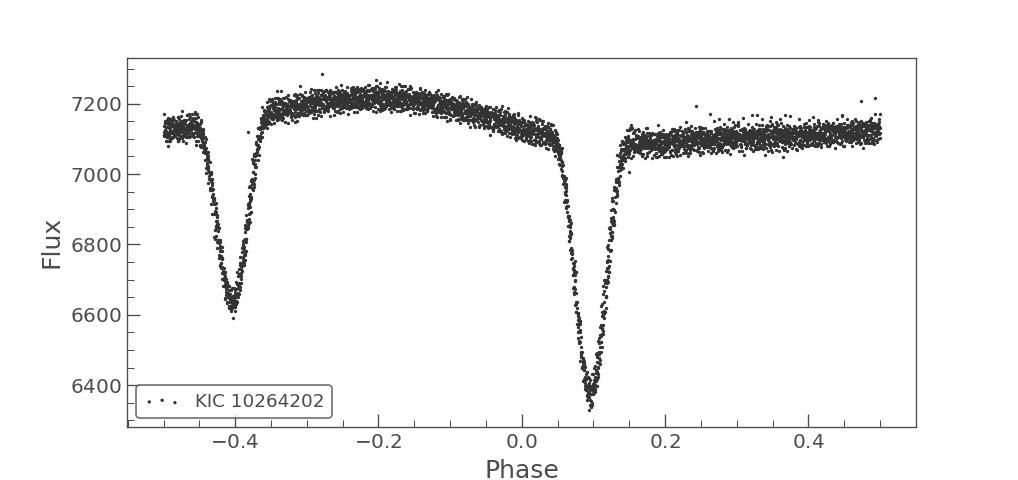
\includegraphics[scale=0.5]{lightcurve.png}
    \caption{Curva de luz de una binaria eclipsante. El flujo del sistema se reduce si es que una de las estrellas oculta a la otra, pero hay una diferencia entre ambos eclipses, donde el flujo se reduce menos si la estrella que se bloquea es la menos brillante.}
    \label{fig:eclipsantes}
\end{figure}
Podemos identificar dos areas en el que el periodograma usado por ALeRCE se puede mejorar:
\begin{enumerate}
    \item {\bf Eficiencia:} La velocidad de ejecución del cálculo de características es de gran importancia, debido a que ALeRCE actualmente usa datos del {\it Zwicky Transient Facility} (ZTF), un sondeo del cielo nocturno que produce 1.4 TB de datos por noche, y el sistema debe ser capaz de mantenerse al ritmo de este volumen de datos. En general, el volumen de datos en la astronomía es cada vez mayor, por ejemplo para el sondeo del LSST, el volumen de datos será cerca de 15 TB por noche, por lo que se debe mejorar continuamente la velocidad de estos algoritmos. Actualmente, MHAOV es uno de los algoritmos que toma más tiempo en el cálculo de características, tomando alrededor del $20\%$ del tiempo.

    La versión de MHAOV se ejecuta en CPU, pero como es posible calcular la medida de confianza para cada frecuencia de prueba y curva de luz independientemente, el algoritmo se podría ver beneficiado de una implementación paralela en GPU, ya que se debe procesar una gran cantidad de curvas de luz y frecuencias.
\begin{figure}[h]
    \centering
    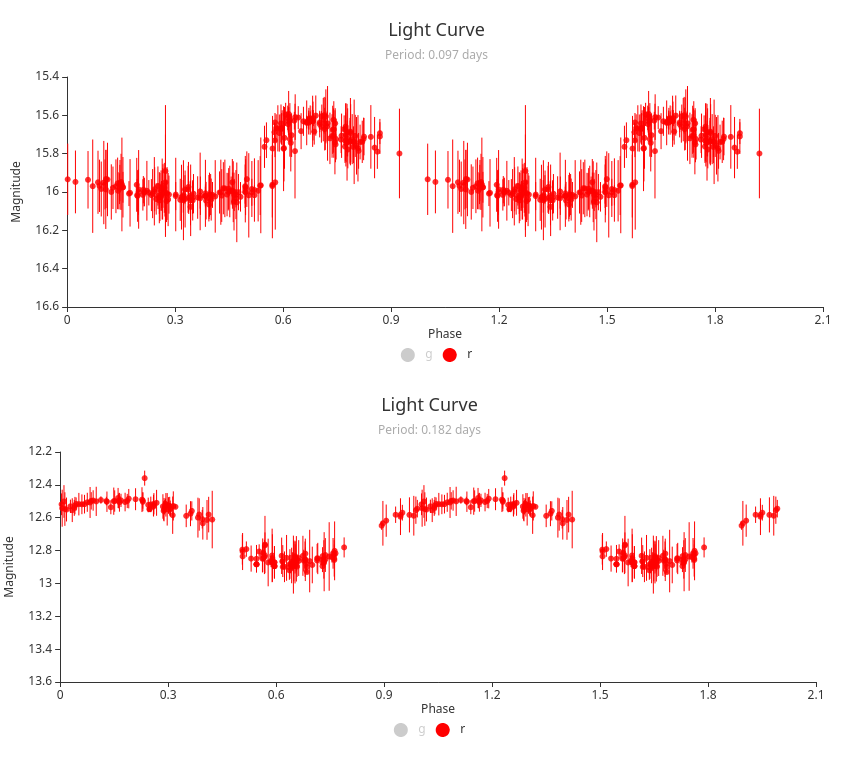
\includegraphics[width=0.8\textwidth]{./figs/scutti-vs-eb.png}
    \caption{Curva de luz de una $\delta$-Scuti (Arriba) y una binaria eclipsante (Abajo). Sus curvas de luz son similares pero sus periodos son muy diferentes (Fuente: \href{https://alerce.online/}{ZTF Explorer})}
    \label{fig:scuti-vs-eb}
\end{figure}
    \item {\bf Precisión:} Hay fuentes para las cuales MHAOV es particularmente impreciso. Específicamente, MHAOV calcula un periodo igual a la mitad del periodo real para gran parte de las binarias eclipsantes, ya que no es lo suficientemente sensible como para distinguir entre ambos eclipses (ver Fig. \ref{fig:binarias}). Esto lleva a que el $2\%$ de las binarias eclipsantes se clasifiquen incorrectamente como estrellas $\delta$-Scuti, ya que estas últimas tienen un rango de periodos menor al de las binarias eclipsantes, pero sus curvas de luz son muy parecidas (ver Fig. \ref{fig:scuti-vs-eb}. Debido a la gran cantidad de binarias eclipsantes, la contaminación en las estrellas $\delta$-Scuti es considerable.

    Esto se podría solucionar considerando otros periodogramas simultáneamente en el clasificador, de manera que este pueda aprender cuando darle más importancia al resultado de uno que del otro y así mejorar la clasificación, o hacer algún otro postproceso que pueda determinar si el resultado de un periodograma es correcto o no. La desventaja de esta solución es el costo computacional: calcular otro periodograma podría incrementar considerablemente el tiempo de ejecución usado por el cálculo de los periodos.
\end{enumerate}
\section{Objetivos}\label{sec:objetivos}
  \subsection*{Objetivo General}\label{sec:obj-g}
  Desarrollar un algoritmo paralelo en GPU que permita determinar el periodo de un gran volumen de fuentes variables en base a sus curvas de luz, con especial énfasis en aumentar la precisión de este para estrellas binarias eclipsantes, de manera que se logre obtener el periodo real y no alguna fracción de este.

  \subsection*{Objetivos Específicos}\label{sec:obj-e}
  Para cumplir el objetivo de la memoria, se deben lograr las siguientes metas:
  \begin{enumerate}
  \item Estudiar y analizar algoritmos para obtener el periodo ya existentes, empezando por GCE y MHAOV.
  \item Implementar una versión paralela en GPU de MHAOV, denominada GMHAOV, complementando el diseño propio con las técnicas de paralelización usadas en GCE.
  \item Validar y comparar el desempeño de los algoritmos, tanto en términos de tiempo de ejecución como en precisión, usando conjuntos de datos con periodo conocido.
  \item Evaluar el impacto de incluir el resultado de más de un periodograma  en el clasificador de ALeRCE.
  \item Verificar que al integrar algoritmo mas preciso  en ALERCE es lo suficientemente eficiente en calcular las características y representa una mejora con respecto al algoritmo actual.
  \end{enumerate}
\section{Plan de Trabajo}\label{chap:sol}

Ya que este trabajo consistió en desarrollar implementaciones eficientes de algoritmos ya existentes, se pasó por una fase de investigación y evaluación para determinar con qué algoritmos se trabajaría y como se mejorarían. Estos algoritmos son:
\begin{itemize}
    \item {\bf MHAOV:} El algoritmo siendo usado actualmente por ALeRCE, es necesario saber que tan preciso es y cual es su tiempo de ejecución a fin de compararlo con otros algoritmos. Para mejorar su velocidad de ejecución, se implementó una versión en GPU de este algoritmo, por lo que es muy importante entenderlo a profundidad para poder implementar GMHAOV.
    \item {\bf GCE:} Un periodograma implementado en GPU que usa entropía condicional, una medida de la correlación entre el magnitud y la fase de una curva de luz doblada, y que es considerablemente más rápido que MHAOV. \ref{gce}
    \item {\bf Métodos de identificar subarmónicos:} A veces, periodogramas como MHAOV identifican subarmónicos del periodo real como se describió en \ref{sec:motivacion}, por lo que es beneficioso investigar algoritmos que ayuden a identificar estas situaciones para poder encontrar el periodo real.
\end{itemize}

Se tomó la decisión de implementar GMHAOV en CUDA, ya que se tenía experiencia con el desarrollo de algoritmos en GPU en este lenguaje, se podía usar el código de GCE como base para poder ejecutar código en CUDA desde python, y además se tenía el hardware necesario para esto. El diseño de GMHAOV se hizo tomando ventaja de que el cálculo de la medida de confianza es independiente entre curvas de luz y frecuencias, y de hecho el mismo diseño de MHAOV permitía paralelizar este cálculo para cada punto de cada curva de luz.

GMHAOV se validó usando el código de generación de curvas de luz disponible en el 
\href{https://github.com/alercebroker/P4J}{repositorio que contiene MHAOV}, y curvas de luz de sets etiquetados (Conjuntos cuyas propiedades son conocidas). Como GMHAOV debe presentar exactamente los mismos resultados que su versión secuencial, bastó con comparar los valores de $\Theta(\omega)$ para ambas versiones y asegurarse que estén lo suficientemente cerca. Usando el generador de curvas de luz, fue posible evaluar el tiempo de ejecución de GMHAOV y compararlo con GCE y MHAOV en función de el número de frecuencias de prueba y número de curvas de luz.

Con respecto a mejorar la precisión del cálculo del periodo, en especial en el caso de las binarias eclipsantes, se implementó un algoritmo que identifica submúltiplos llamado promediado de subarmónicos, que permite discriminar entre señales falsas y señales reales en el periodograma, pero requiere ordenar los valores de $\Theta$ para todas las frecuencias de prueba. Se evalúa el impacto de este postproceso en la precisión del periodograma y además su velocidad de ejecución.

Para estudiar el impacto de los algoritmos implementados en el clasificador, se planea entrenar el clasificador de ALeRCE incluyendo como características el resultado de GMHAOV, GCE y del promediado de subarmónicos. Con esto se espera evaluar el impacto de agregar los resultados de otros clasificadores, en especial con respecto a las binarias eclipsantes.

\section{Contenido de la memoria}\label{chap:contenido}
\begin{itemize}
    %\item   {\bf Antecedentes:} Se explican los fundamentos de la computación en GPU, la arquitectura y su modelo de memoria.
    \item {\bf Análisis del software:} Se hace un análisis profundo del software que se usó como base en el desarrollo de la solución, incluyendo comparaciones entre sus precisiones y rendimientos. 
    \item {\bf Diseño:} Se describe el diseño de la solución, incluyendo el desarrollo de la interfaz en Python para ejecutar el código de CUDA, el proceso de paralelización de MHAOV y el diseño de un postproceso al periodograma que es capaz de identificar señales falsas.
    \item {\bf Implementación:} Se muestra la implementación de la solución, explicando en detalle y con secciones de código como se llevó a cabo el diseño del capítulo anterior.
    \item {\bf Resultados:} Se describen los métodos de evaluación del rendimiento y precisión de la solución, y se presentan sus resultados y comparaciones con la versión secuencial de MHAOV y el impacto del postproceso que identifica señales falsas en el periodograma.
    \item {\bf Análisis y conclusión:} Se realiza un análisis de los resultados expuestos en la sección anterior, se realizan conclusiones respecto a los objetivos en función de esto y se discute el trabajo futuro.
\end{itemize}

%\chapter{Antecedentes}\label{chap:anteceddentes}
%\section{Paralelización en GPU}\label{sec:paralelizacion}
%\section{Arquitectura de CUDA}\label{sec:arquitectura-cuda}
%\section{Modelo de memoria de CUDA}\label{sec:modelo-memoria}
%\section{Reducción en GPU}\label{sev:reduccion}

\chapter{Análisis del software}\label{chap:analisis}

En este capítulo, se detallan los detalles del pipeline de ALeRCE y de los algoritmos estudiados durante el curso de la memoria, empezando por MHAOV, GCE y la comparación entre estos dos.

\section{El pipeline de ALeRCE}\label{sec:alerce-pipeline}
El sistema de ALeRCE recibe un flujo de aletas desde ZTF, que contiene varios datos de la observación como la magnitud en distintas bandas y su posición. Estos datos se procesan de la siguiente manera, como se observa en la figura \ref{fig:pipeline} \cite{lightcurve-classifier}
\begin{enumerate}
    \item  {\bf S3 upload:} Se suben los paquetes de alertas al servicio de almacenamiento de AWS S3 para uso posterior.
    \item {\bf Cross match:} Se usa la posición de la alerta para buscar coincidencias con catálogos externos y obtener más información sobre el objeto.
    \item {\bf Stamp classifier:} La imagen de los objetos nuevos son clasificadas.
    \item {\bf Preprocessing:} Se hacen correcciones a la magnitud y se calculan estadísticas simples de las curvas de luz.
    \item {\bf Light curve features:} Se calculan estadísticas avanzadas para curvas de luz con más de 6 puntos, incluyendo el periodo.
    \item {\bf Light curve classifier:} Se clasifica el objeto usando las características calculados y a los datos del objeto adquiridos en el crossmatch.
    \item {\bf Outliers:} Se aplica un algoritmo de detección de outliers para identificar curvas de luz que pueden ser particularmente interesantes.
    \item {\bf ALeRCE stream:} Se reportan las curvas de luz en un stream incluyendo su clasificación y las características calculadas.
\end{enumerate}
\begin{figure}[H]
    \centering
    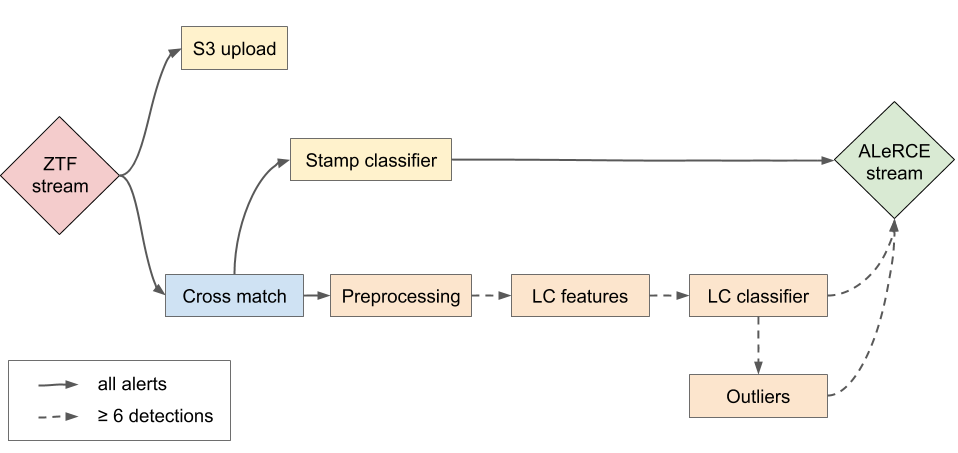
\includegraphics[scale=0.45]{pipeline.png}
    \caption{Pipeline de ALeRCE \cite{alerce-intro}. Entre el procesamiento que se le hace al stream de alertas de ZTF, está el tratamiento a las curvas de luz, donde después de una corrección, se calculan características que serán usadas para la clasificación de las curvas de luz.}
    \label{fig:pipeline}
\end{figure}
\section{Arquitectura de MHAOV}\label{sec:arquitectura-mhaov}
MHAOV usa como medida de confianza que tan bien se ajusta un sinusoide con un determinado número de armónicos a la forma de la curva. En su base, consiste en asumir que las observaciones $X$ son la suma de la señal $F$ y el error $E$, de tal manera que la observación $k$ es $X_k= F_k+E_k$. La forma de la señal $F^{(N)}$ es de una serie de fourier con $N$ armónicos. Con el fin de descomponer la señal en sus componentes, definimos el polinomio $\Psi_{2N}(z)$, de manera de que para una frecuencia de prueba $\omega$, los argumentos del polinomio tienen la forma $z_k = e^{i \omega}$, y se asocian a la $k$-ésima observación, y su valor para $z_k$  es $\Psi_{2N}(z_k)=z_k^N F(t_k)$). Notamos que en un espacio de Hilbert un polinomio de grado $N$ puede ser descompuesto en función de una base ortonormal del espacio $\{\Phi\}_{n=1,..,N}$
\begin{align}
    \Psi_N(z) &= \sum_{n=1}^{N} c_n \Phi_n(z)
.\end{align}
Donde el producto interno está definido como
\begin{align}
    (\Phi, \Psi) &= \sum_{k=1}^{K} g_k \Phi(z_k) \overline {\Psi(z_k)} \label{eq:scalar-product}\\
    g_k &\approx \frac{1}{\mbox{Var}\{X_k\}} \nonumber 
.\end{align}
Esta base se puede obtener de manera iterativa
\begin{align}
    \tilde{ \Phi }_0(z)  &= 1 \\
    \tilde{ \Phi }_{n+1}(z)  &= z \tilde{ \Phi}_n-\alpha_n z^n \overline{\tilde{\Phi}_n(z) } \label{eq:recurrence} \\ 
\Phi_n(z) &= \frac{\tilde{ \Phi}_n(z) }{\sqrt{(\tilde{\Phi}_n, \tilde{\Phi}_n)}}\\
\alpha_n &= \frac{(z\tilde{\Phi}_n, \tilde{\Phi}_n }{(z^n \overline{\tilde{\Phi}_n}, \tilde{\Phi}_n)} \label{eq:alpha} \\
c_n &= \frac{(\Psi, \tilde{\Phi}_n)}{\sqrt{(\tilde{\Phi}_n, \tilde{\Phi}_n)}} \label{eq:c}
.\end{align}
Para el MHAOV, la medida de confianza se basa en estimadores de la varianza de $F$ y $E$, y es $\Theta \equiv \widehat{\mbox{Var}} \{F\}/\widehat{\mbox{Var}} \{E\}$, que tiene la forma (Para mas detalle ver \cite{MHAOV})
\begin{align}
    \Theta(\omega) &= \frac{(K - 2N - 1) \sum_{n=0}^{2N} |c_n|^2}{2N[(X,X)- \sum_{n=0}^{2N} |c_n|^2]} \label{eq:theta} 
.\end{align}
El procedimiento para calcular la medida de confianza es entonces el siguiente:
\begin{enumerate}
    \item Fijar los valores iniciales para la recurrencia, $n=-1$, $\tilde{\Phi}_{-1} = 1/z$, y $\alpha_{-1}=0$.
    \item Usar \eqref{eq:recurrence} para encontrar el siguiente valor de $\tilde{\Phi}_n$
    \item Usar \eqref{eq:scalar-product} para calcular los valores de \eqref{eq:alpha} y \eqref{eq:c}.
    \item Volver al paso 2, iterando esto $N$ veces.
    \item Calcular $\Theta(\omega)$ usando \ref{eq:theta}.
\end{enumerate}
    
\begin{algorithm}[H]
\caption{MHAOV}\label{alg:mhaov}
\begin{algorithmic}
    \State $wmean \gets \text{weighted\_mean}(mag, err, N)$ \Comment{weighted mean}
\For{$i \gets 1$ to $N$}
\State $wvar \gets wvar + (mag[i] - wmean)^{2}/err[i]^{2}$ \Comment{weighted variance $(X, X)$}
\EndFor
\State $\Theta \gets 0$
\For{\texttt{$i \gets 1$ to $N$}}\Comment{Inicialización de variables}
    \State $\phi \gets 2 \pi (mjd[i]*\omega - \floor{mjd[i]*\omega})$
    \State $z_r = \cos(\phi)$ \Comment{Inicialización de $z$}
    \State $z_i = \sin(\phi)$ 
    \State $zn_r = 1$ 
    \State $zn_i = 0$
    \State $p_r = 1/err[i]$
    \State $p_i = 0$
    \State $cf_r = (mag[i] - wmean)\cos(K * \phi) / err[i]$
    \State $cf_i = (mag[i] - wmean)\sin(K * \phi) / err[i]$
\EndFor
\For{$j \gets 1$ to 2$K + 1$}
    \State $sn, al_r, al_i, sc_r, sc_i \gets 0$

        \For{\texttt{$i \gets 1$ to $N$}}
    \State $sn \gets sn + {p_r}^{2}+ {p_i}^{2}  $
    \State $al_r \gets al_r (z_r[i] \cdot  p_r[i] - z_i[i] \cdot  p_i[i])/err[i]$ \Comment{Siguiente valor de de $\alpha$}
        \State $al_i \gets al_i + ( z_r[i] \cdot  p_i[i] + z_i[i] \cdot  p_r[i])/err[i]$
        \State $sc_r \gets sc_r + p_r[i] \cdot  cf_r[i] + p_i[i] \cdot  cf_i[i]$ \Comment{Siguiente valor de $c$}
        \State $sc_i \gets sc_i + p_r[i] \cdot  cf_i[i] - p_i[i] \cdot  cf_r[i]$
    \EndFor
    \State $sn \gets \max(sn, 10\cdot {-9})$
    \State $al_r \gets al_r/sn$
    \State $al_i \gets al_i/sn$
    \State $\Theta \gets \Theta + ({sc_r}^{2} + {sc_i}^{2})/sn$
    \For{$i \gets 1$ to $N$}
        \State $s_r \gets al_r \cdot zn_r[i] - al_i \cdot zn_i[i]$
        \State $s_i \gets al_r \cdot zn_i[i] + al_i \cdot zn_r[i]$
        \State $tmp \gets p_r[i]\cdot z_r[i] - p_i[i]\cdot z_i[i] - s_r\cdot p_r[i] - s_i\cdot p_i[i]$
        \State $p_i \gets p_r[i]\cdot z_i[i] - p_i[i]\cdot z_r[i] - s_r\cdot p_i[i] - s_i\cdot p_r[i]$ \Comment{Actualizar el valor de $\Phi_n$}
        \State $p_r \gets tmp$
        \State $tmp \gets zn_r[i] \cdot z_r[i] - zn_i[i] \cdot z_i$
        \State $zn_i \gets zn_i[i] \cdot z_r[i] + zn_r[i] \cdot z_i$ \Comment{Actualizar el valor de $z^{n}$}
        \State $zn_r \gets tmp$
    \EndFor
\EndFor
\State \Return $(K-2N-1)\cdot \Theta / (2N\cdot \text{max}(wvar - \Theta, 10^{-9}))$

\end{algorithmic}
\end{algorithm}

\section{Arquitectura de GCE}\label{sec:gce}
\section{Comparación de MHAOV vs GCE}\label{sec:mhaov-vs-gce}
Se realizó una comparación de MHAOV y GCE usando tests previamente escritos por Pablo Huijse, usando sets etiquetados, que son archivos con información sobre objetos, incluyendo su clase y periodo. Los tests miden el tiempo de ejecución y la precisión de cada algoritmo usando curvas de luz con mas de 20 puntos en sus curvas de luz, y fueron realizados en un computador con un procesador Intel Core i7-9750H de 12 núcleos lógicos y una GPU Nvidia GeForce 1660 Ti con 6GB de memoria. MHAOV fue ejecutado con $8$ threads en paralelo.

Para el primer test, se usaron alrededor de 8500 estrellas RR Lyrae, que tienen curvas suaves y periodos marcados, y en las tablas \ref{table:tiempos-rrl} y \ref{table:precision-rrl} se encuentran los resultados.
\begin{table}[H]
\caption{Tiempos de ejecución total y por curva para ambos algoritmos, usando el mismo conjunto de datos.}
    \begin{tabular}{|c|c|c|}
    \hline
    Algoritmo & Tiempo de ejecución {[}s{]} & Tiempo por curva {[}ms{]} \\ \hline
    GCE       & 85                          & 32                        \\ \hline
    MHAOV     & 629                         & 242                       \\ \hline
    \end{tabular}
    \label{table:tiempos-rrl}
\end{table}

\begin{table}[H]
\caption{Clasificación en porcentajes para los valores del periodo calculado respecto al real. Acierto significa que estos sin similares, Múltiplo que el calculado es un múltiplo del original, Submúltiplo que es una fracción del original, Alias que es un alias del original (Es decir, que se ajusta igualmente bien a los datos debido a su naturaleza discreta), y Otro para cualquier otro valor del periodo calculado.}
\begin{tabular}{|c|c|c|c|c|c|}
    \hline
    Algoritmo & Acierto & Múltiplo & Submúltiplo & Alias & Otro \\ \hline
    GCE       & 69.5  & 1.7      & 1.8         & 1.7   & 25.3  \\ \hline
    MHAOV     & 88.8  & 1.0      & 0.2         & 1.1   & 8.7   \\ \hline
    \end{tabular}
    \label{table:precision-rrl}
\end{table}
La segunda prueba se hizo con binarias eclipsantes, y la comparación de la precisión de ambos algoritmos está en la tabla \ref{table:precision-eb}. Notemos que si multiplicamos los periodos obtenidos por $2$, los resultados cambian a los resultados de la tabla \ref{table:precision-corrected}, pero aún así observamos cierto grado de contaminación, y al hacer esto estamos obteniendo el periodo equivocado para binarias eclipsantes donde la diferencia de periodos es significativa.


\begin{table}[H]
\caption{Clasificación en porcentajes para los valores del periodo calculado respecto al real para las binarias eclipsantes.}
\begin{tabular}{|c|c|c|c|c|c|}
    \hline
    Algoritmo & Acierto & Múltiplo & Submúltiplo & Alias & Otro \\ \hline
    GCE     & 0.42  & 93.30      & 0.00         & 0.00   & 6.28   \\ \hline
    MHAOV       & 11.1  & 55.14      & 0.32         & 0.56   & 32.92  \\ \hline
    \end{tabular}
    \label{table:precision-eb}
\end{table}

\begin{table}[H]
\caption{Comparación entre ambos algoritmos para las tres situaciones: usando RR Lyrae, binarias eclipsantes, y multiplicando por $2$ el periodo obtenido por los algoritmos para binarias eclipsantes.}
\begin{tabular}{|c|c|c|c|c|}
\hline
Prueba & \begin{tabular}[c]{@{}c@{}}Ambos\\ aciertan\\ {[}\%{]}\end{tabular} & \begin{tabular}[c]{@{}c@{}}MHAOV acierta,\\ GCE no {[}\%{]}\end{tabular} & \begin{tabular}[c]{@{}c@{}}GCE acierta,\\ MHAOV no\\ {[}\%{]}\end{tabular} & \begin{tabular}[c]{@{}c@{}}Ninguno\\ acierta \\ {[}\%{]}\end{tabular} \\ \hline
RR Lyrae & 61.40 & 27.40 & 3.40 & 7.78 \\ \hline
\begin{tabular}[c]{@{}c@{}}Binarias\\ Eclipsantes\end{tabular} & 0.20 & 0.22 & 10.86 & 88.72 \\ \hline
\begin{tabular}[c]{@{}c@{}}Binarias\\ Eclipsantes\\ (Ajustado)\end{tabular} & 10.46 & 82.46 & 0.60 & 6.48 \\ \hline
\end{tabular}
\end{table}




\begin{table}[H]
\caption{Precisión de MHAOV después de multiplicar los periodos obtenidos por $2$}
\begin{tabular}{|c|c|c|c|c|c|}
    \hline
    Algoritmo & Acierto & Múltiplo & Submúltiplo & Alias & Otro \\ \hline
    2 $\cross$ GCE       & 54.50  & 0.30      & 11.88         & 1.30   & 32.02  \\ \hline
    2 $\cross$ MHAOV       & 92.92  & 0.32      & 0.42         & 0.14   & 6.20  \\ \hline
    \end{tabular}
    \label{table:precision-corrected}
\end{table}

Notamos que GCE, aunque es considerablemente más rápido que MHAOV, es significativamente menos preciso, incluso para el caso de submúltiplos, donde se esperaba que redujera estos casos ya que es un algoritmo que no ajusta una sinusoidal a diferencia de MHAOV. Además, el aporte de GCE con respecto a calcular el periodo de curvas correctamente donde MHAOV no lo hace es pequeño para las RR Lyrae, solo $3.4\%$ y $0.60\%$ para las binarias eclipsantes, pero esto puede ser significativo por la gran cantidad de binarias eclipsantes que hay. Se concluye a partir de estas pruebas que no se puede simplemente reemplazar MHAOV por GCE en ALeRCE, ya que se perderá demasiada precisión, pero implementar una versión paralela de MHAOV tan rápida como GCE y tan precisa como MHAOV resultará beneficioso.

%\section{Promediado de subarmónicos}\label{sec:subarmonicos-analisis}




\chapter{Diseño}\label{chap:diseño}
A continuación se detalla el detalle del diseño de la solución, empezando por explicar el proceso de paralelización de MHAOV y luego el detalle del algoritmo de promediado de subarmónicos.

\section{Ejecución de código de CUDA usando python}\label{sec:python-cuda}
Ejecutar código de CUDA directamente desde python requiere del paquete \texttt{cupy}, para enviar las curvas de luz a la memoria de la GPU, y de \texttt{cython}, para realizar llamadas a la función en $C$ que ejecuta el kernel desde python. Para poder compilar el código, se debe escribir un script en python que incluya correctamente las librerias, cambiar el método de compilación para incluir CUDA y que indique las arquitecturas para las cuales se debe realizar la documentación. Afortunadamente, el código de GCE tiene una estructura muy similar a la que se planeaba, ya que GCE ofrece una interfaz en python desde la cual se pueden hacer llamadas al kernel, por lo que se usó el código de GCE como base para el script de compilación y para la clase de python encargada de la preparación de los datos para ser enviados a la memoria de la GPU.

\section{Paralelización de MHAOV}\label{sec:paralelización}
Como se expuso en la sección \ref{sec:motivacion}, MHAOV puede ser paralelizado a nivel de las curvas de luz y las frecuencias de prueba, ya que los valores $\Theta(\omega)$ son independientes entre sí. Adicionalmente, de la descripción del algoritmo en la sección \ref{sec:arquitectura-mhaov} se observa que los ciclos que iteran por el largo de la curva de luz también se pueden paralelizar, para el primer y segundo ciclo la paralelización es trivial, y para el segundo ciclo se puede calcular el aporte de cada ciclo a los valores de las variables, y luego usar reducción para sumar estos aportes y usar los resultados para calcular el incremento en $\Theta$ y para el tercer ciclo que una vez más es trivialmente paralelizable ya que los ciclos no dependen entre sí.

Así, se requiere coordinar los threads en ciertos puntos del kernel para evitar data races, y a continuación se presenta el pseudo-código del kernel de GMHAOV, siendo análogo al código presentado en \ref{sec:arquitectura-mhaov}:

\begin{algorithm}[H]
\caption{GMHAOV}\label{alg:gmhaov}
\begin{algorithmic}
    \Function{GMAHOVKernel}{$lc_i$, $\omega_i$, $i$}
    \If{$i == 0$}
        \State $\Theta \gets 0$
    \EndIf
    \State $wmean \gets$ cálculo paralelo de los aportes de cada punto y suma por reducción 

    \_\_syncthreads()
    \State $wmvar \gets$ cálculo paralelo de los aportes de cada punto y suma por reducción 

    \_\_syncthreads()
    \State $z_r, \ z_i, \ z_n, \ p_r, \ p_i, \ cf_r, \ cf_i \gets$ valores inciales según $mjd[lc_i, i]$, $err[lc_i, i]$ y $mag[lc_i, i]$

    \_\_syncthreads()
    \For{$j \gets 0$ to $2K + 1$}
        \State $al_r, \ al_i, \ sc_r, \ sc_i, \ sn \gets$ suma de los aportes de cada punto por reducción

    \_\_syncthreads()
        \If{$i == 0$}
            \State $\Theta \gets \Theta + ({sc_r}^{2} + {sc_i}^{2})/sn$
        \EndIf
        \State $s_r, \ s_i, \ p_r, \ p_i, \ zn_i, \ zn_r \gets$ Valores actualizados usando $al_r, \ al_i, \ zn_r, \ zn_i, \ p_r, \ p_i, \ z_r$ y  $z_i$

    \_\_syncthreads()
    \EndFor

    \_\_syncthreads()
\State  $\Theta \gets (K-2N-1)\cdot \Theta / (2N\cdot \text{max}(wvar - \Theta, 10^{-9}))$
    \EndFunction
\end{algorithmic}
\end{algorithm}

Como las curvas de luz son independientes entre sí y estas tienen en promedio $150$ puntos, se pueden guardar completamente en memoria compartida para cada bloque y así solo acceder a memoria global solo para obtener las curvas y su número de puntos. Además de las curvas de luz, se deberá usar la memoria local para la reducción de 8 variables, usando 8 arreglos del largo de la curva de luz más larga. 

\section{Promediado de subarmónicos}\label{sec:subarmonicos-diseno}
El promediado de subarmónicos es descrito en \cite{graham-entropy}, pero el código no está disponible así que se tuvo que diseñar este algoritmo en base a la descripción en el paper citado. La idea del promediado de subarmónicos, es que si en el periodograma se tiene una señal real en $\Theta(\omega)$, entonces el periodograma tendrá un peak relevante en $\frac{\omega}{2}$. De esta manera, si se promedia el valor de $\Theta$ en $\omega$ y en $\frac{\omega}{2}$, se debe seguir teniendo un valor significativo, de lo contrario se tenía una señal falsa y la frecuencia real está en otra parte.

Para poder implementar esto como algoritmo, es necesario ordenar los valores de $\Theta$ para obtener las frecuencias más relevantes. El costo computacional de esto se puede reducir buscando maximos o mínimos locales de $\Theta$ escaneando el arreglo de valores y marcando aquellos que son mayores que sus vecinos, lo cual tiene un costo computacional de $\mathcal O(N_\omega)$, con $N_\omega$ la cantidad de frecuencias de prueba, y luego ordenando estos valores. El costo computacional seguirá siendo de $\mathcal O (N_\omega \ln N_\omega)$, pero el ordenamiento podrá ignorar la gran mayoría de las frecuencias. Luego se elijen las frecuencias con mayor valor de $\Theta$, y se marcan como señales significantes.

Se establece un criterio simple para determinar si una señal significante es real: Si existe otra señal significante cerca de la mitad de su frecuencia asociada, entonces se promedian los valores de $\Theta$ y se le asigna como puntaje a la frecuencia. Si no existe esta señal, entonces su puntaje es nulo. Así se elije la frecuencia asociada a la señal con el mayor puntaje y se eliminan las señales falsas. Asociarle este puntaje al resultado del periodograma es conveniente pues se puede usar posteriormente como característica del clasificador.

\chapter{Implementación}\label{chap:implementación}
En este capítulo se detalla la implementación de la solución, empezando por como se preparan los datos en python para ser cargados en la memoria de la GPU, la implementación del kernel y finalmente el promediado de subarmónicos.
\section{Preparación de los datos en python}\label{sec:preparacion-datos}
Se crea la clase de python GMHAOV, basada en GCE, con una función que recibe las curvas de luz, las frecuencias de prueba y el tamaño de batch, según el cual se dividen las curvas de luz y se mandan en partes para no sobrecargar la memoria. Se ignoran varias funciones de GCE que no se reimplementaron en GMHAOV.
\begin{lstlisting}[language=Python]
def batched_run_const_nfreq(self, lightcurves, batch_size, freqs):
...
    # split by light curve batches
    split_inds = []
    i = 0
    while i < len(lightcurves):
        i += batch_size
        if i >= len(lightcurves):
            break
        split_inds.append(i)

    lightcurves_split_all = np.split(lightcurves, split_inds)
...
    bf = []
    per_vals = []
    for i, light_curve_split in iterator:

        # run one light curve batch
        out = self._single_light_curve_batch(
            light_curve_split,
            freqs)
...
\end{lstlisting}
Como se usa CUDA para el procesamiento de las curvas de luz, es necesario determinar el largo de cada curva de luz y el largo máximo, para que se pueda realizar el cálculo del periodograma sin considerar datos que pueden contaminar las curvas de luz y para poder determinar el tamaño que cada bloque debe tener, pues estos deben tener a lo menos un thread por punto de la curva de luz. Luego se crean arreglos para los tiempos, magnitudes y errores para las curvas de luz, donde cada curva tiene un largo equivalente al de la curva más larga, y las entradas adicionales se rellenan con $0$s.

Originalmente, GCE realizaba otros cálculos relacionados al binning de las magnitudes y los tiempos, además de considerar los valores de $\dot p$, pero esto fue removido y el código fue adaptado para funcionar sin esto.
\begin{lstlisting}[language=Python]

# determine maximum length of light curves in batch
# also find minimum and maximum magnitudes for each light curve
max_length = 0
number_of_pts = np.zeros((len(light_curve_split),)).astype(int)
for j, lc in enumerate(light_curve_split):
    number_of_pts[j] = len(lc)
    max_length = max_length if len(lc) < max_length else len(lc)
light_curve_arr = np.zeros((len(light_curve_split), max_length, 3))
logging.info(f"Number of points {number_of_pts}")

# populate light_curve_arr
for j, lc in enumerate(light_curve_split):
    light_curve_arr[j, : len(lc)] = np.asarray(lc)

# separate time and mag info
light_curve_times = light_curve_arr[:, :, 0]

light_curve_mags = light_curve_arr[:, :, 1]

light_curve_errs = light_curve_arr[:, :, 2]
\end{lstlisting}

Luego se aplanan los arreglos para formar tres arreglos muy largos, y se cargan en la memoria de la GPU usando la función de cupy \texttt{xp.asarray} junto con el arreglo con las frecuencias de prueba, el arreglo que contendrá los resultados del periodograma y el arreglo que contiene el número de armónicos con el que se correrá el periodograma para cada curva. Luego se llama al envoltorio de la función que llama al kernel con los arreglos creados y otros datos como el número de frecuencias y el número de curvas de luz.
\begin{lstlisting}[language=Python]
        # flatten everything
        light_curve_times_in = (
            xp.asarray(light_curve_times).flatten().astype(self.dtype)
        )

        light_curve_mags_in = xp.asarray(light_curve_mags.flatten()).astype(
            self.dtype
        )

        light_curve_errs_in = xp.asarray(light_curve_errs.flatten()).astype(
            self.dtype
        )
        number_of_pts_in = xp.asarray(number_of_pts).astype(xp.int32)

        freqs_in = xp.asarray(freqs).astype(self.dtype)

        per_vals_out_temp = xp.zeros(
            (len(freqs_in) * len(light_curve_times),), dtype=self.dtype
        )

        max_num_pts_in = number_of_pts_in.max().item()
        Nharmonics = xp.ones(len(light_curve_times), dtype=xp.int32)

        self.gmhaov_func(
            per_vals_out_temp,
            freqs_in,
            len(freqs_in),
            light_curve_times_in,
            light_curve_mags_in,
            light_curve_errs_in,
            number_of_pts_in,
            Nharmonics,
            len(light_curve_times),
            max_num_pts_in
        )
        per_vals_out_temp = per_vals_out_temp.reshape(
            len(light_curve_times), len(freqs_in)
        )
\end{lstlisting}
En la última linea se cambia la forma del arreglo con los resultados del periodograma de manera que sea un arreglo de los valores de $\Theta$ para cada curva de luz.
El envoltorio de la función que llama al kernel está escrito en Cython, y usa una decoración que reemplaza los arreglos que recibe la función como argumentos por sus punteros en memoria. En este caso, como los arreglos están en memoria de la GPU, estos son reemplazados por los punteros a su localización en la GPU. Luego, la función en CUDA \texttt{run\_gmhaov}, encargada de hacer las llamadas al kernel, es ejecutada con estos punteros como argumentos.
\begin{lstlisting}[language=Python]
@pointer_adjust
def run_gmhaov_wrap(per, freqs, num_freqs, mjds, mags, errs, num_pts_arr, Nharmonics_arr, num_lcs, num_pts_max,  wmeans_arr, wvars_arr):
    cdef size_t per_in = per
    cdef size_t freqs_in = freqs
    cdef size_t num_freqs_in = num_freqs
    cdef size_t mags_in = mags
    cdef size_t mjds_in = mjds
    cdef size_t errs_in = errs
    cdef size_t num_pts_arr_in = num_pts_arr
    cdef size_t Nharmonics_arr_in = Nharmonics_arr
    cdef size_t num_lcs_in = num_lcs
    cdef size_t num_pts_max_in = num_pts_max
    run_gmhaov(<fod *> per_in, <fod *> freqs_in, num_freqs_in, <fod *> mags_in, <fod *> mjds_in, <fod *> errs_in,
                             <int *> num_pts_arr_in, <int *> Nharmonics_arr_in, num_lcs, num_pts_max_in, <float *> wmeans_arr_in, <float *> wvars_arr_in)
\end{lstlisting}
\section{Paralelización}\label{sec:paralelización-implementacion}
Como la memoria local usada por cada bloque es dinámica, y los arreglos relevantes ya están en la memoria de la GPU, \texttt{run\_gmhaov} es una función relativamente corta, pues no necesita mover objetos desde la memoria del host a la del dispositivo. El tamaño ded la grilla se escoje como el número de frecuencias en el eje $x$ y el número de curvas de luz en el eje $y$, y la memoria de cada bloque es el espacio que ocupará cada curva de luz más los arreglos necesarios para hacer las reducciones descritas en \ref{sec:paralelizacion}.

Como siempre es conveniente tener potencias de $2$ como tamaño de bloque, se aproxima el largo máximo de las curvas de luz a su próxima potencia de $2$ y se elije esto como tamaño de bloque, con un valor máximo de $1024$, de manera que cada bloque pueda procesar completamente cada curva de luz. Para curvas de luz con más de $1024$ puntos, el kernel se debería encargar de cubrir toos los puntos.
\begin{lstlisting}[language=C]
void run_gmhaov(fod *d_per, fod *d_freqs, int num_freqs, fod *d_mag, fod *d_mjd, fod *d_err,
                 int *num_pts_arr, int *Nharmonics_arr, int num_lcs, int num_pts_max, float *wmeans_arr, float *wvars_arr){
    dim3 griddim(num_freqs, num_lcs, 1); 

    // determine shared memory allocation size
    size_t numBytes = sizeof(fod)*num_pts_max + // magnitude values
                      sizeof(fod)*num_pts_max + // error values
                        sizeof(fod) * num_pts_max + // time values
                        5 * sizeof(fod) * num_pts_max + // sn, scr, sci, alr, ali to sum
                        3 * sizeof(fod) * num_pts_max; // wvar, wmean, w_sum to sum

    int v = num_pts_max;
    // Source for rounder: https://graphics.stanford.edu/~seander/bithacks.html#RoundUpPowerOf2
    v--;
    v |= v >> 1;
    v |= v >> 2;
    v |= v >> 4;
    v |= v >> 8;
    v |= v >> 16;
    v++;
    if (v > 1024) v = 1024;
    kernel<<<griddim, v, numBytes>>>(d_per,
                                                d_freqs, num_freqs,
                                                d_mag, d_mjd,
                                                d_err, num_pts_arr,
                                                Nharmonics_arr, num_lcs,
                                                num_pts_max, wmeans_arr, wvars_arr);
    cudaDeviceSynchronize();
    gpuErrchk(cudaGetLastError());
}
\end{lstlisting}

El kernel empieza por crear el arreglo compartido \texttt{mag\_share}, que tiene el espacio necesario para guardar todos los arreglos locales que se usan en cada bloque. Se definen entonces el resto de los arreglos como punteros a las secciones que le corresponden en memoria, listos para ser rellenados por los datos en memoria global, y finalmente se declaran las cantidades que se comparten en todo el bloque.

\begin{lstlisting}[language=C++]
    
__global__ void kernel(fod* __restrict__ d_per,
                        fod* d_freqs, int num_freqs,
                        fod* d_mag, fod* d_mjd,
                        fod* d_err, int* num_pts_arr,
                        int* Nharmonics_arr, int num_lcs,
                        int num_pts_max, fod* wmeans_arr, fod* wvars_arr)
    {
    /* Assign the magnitude,error and time values to sections of the shared array */
    extern __shared__ fod mag_share[];
    fod *error_share = (fod*) &mag_share[num_pts_max];
    fod *time_share = (fod*) &error_share[num_pts_max];

    fod *sn_sum = (fod*) &time_share[num_pts_max];

    fod *scr_sum = (fod*) &sn_sum[num_pts_max];
    fod *sci_sum = (fod*) &scr_sum[num_pts_max];
    ...
    __shared__ fod sn;
    __shared__ fod scr;
    __shared__ fod sci;
    ...
\end{lstlisting}
En caso de que se haya elegido un tamaño de grilla en el eje $y$ menor al número de curvas de luz, se introduce un ciclo que se asegura que todas las curvas de luz sean procesadas, empezando por $lc_i = \text{blockIdx.y}$. Luego se carga en memoria la curva de luz actual de forma paralela, y se itera en frecuencias en el eje $x$ de la misma manera que se hace en el eje $y$, empezando por $f_i = \text{blockIdx.x}$. Se definen las variables que se usarán para el cálculo de $\Theta$, y uno de los threads inicializa a $\Theta=0$.
\begin{lstlisting}[language=C++]
    for (int lc_i = blockIdx.y; lc_i < num_lcs; lc_i += gridDim.y){
        int num_pts_current = num_pts_arr[lc_i];
            int current_index = lc_i * num_pts_max + i;
            mag_share[i] = d_mag[current_index];
            error_share[i] = d_err[current_index];
            time_share[i] = d_mjd[current_index]; 
        }
        __syncthreads();
        for (int fi = blockIdx.x; fi < num_freqs; fi += gridDim.x) {
            int idx = threadIdx.x;
            fod zr, zi, znr, zni, pr, pi, cfr, cfi;

            if (idx == 0) aov = 0;
            ...
\end{lstlisting}
Un problema con la implementación de GMHAOV es que si la curva de luz tiene un largo mayor que el tamaño de bloque máximo de $1024$, no es posible cubrirla en el periodograma y el algoritmo deja de funcionar. El algoritmo toma $i=idx$, el $id$ del thread en el bloque, y calcula $wmean$ y $wvar$ encontrando el aporte de cada valor a estos valores y luego usando reducción para encontrar sus valores finales.
\begin{lstlisting}[language=C++]
            ...
            w_sum_sum[i] = 1.0 / powf(abs(error_share[i]), 2.0f);
            w_mean_sum[i] = mag_share[i] / powf(abs(error_share[i]), 2.0f); }
            __syncthreads();
            for(int size = NUM_THREADS/2; size > 0; size/=2){
                if(idx < size && (idx + size < num_pts_arr[lc_i])){
                    w_sum_sum[idx] += w_sum_sum[idx + size];
                    w_mean_sum[idx] += w_mean_sum[idx + size];
                }
                __syncthreads();
            }

            if (idx == 0) {
                w_sum = w_sum_sum[0];
                w_mean = w_mean_sum[0];
                w_mean = w_mean / w_sum;
                wmeans_arr[lc_i] = w_mean;
            }
            __syncthreads();
            ...
\end{lstlisting}
Luego se procede de forma análoga al pseudocódigo presentado en \ref{sec:arquitectura-mhaov}, con la diferencia principal siendo que el algoritmo calcula el aporte de cada punto a los valores de $\alpha$, $c$ y $sn$ y los usa para obtener sus valores finales usando reducción. Es necesario sincronizar el bloque después de inicializar las variables, al terminar de calcular los aportes de cada punto, como parte de la reducción, y después de calcular el aporte del ciclo a $\Theta$.
\begin{lstlisting}[language=C++]
        fod arg = d_freqs[fi] * time_share[i];
            fod phi = 2 * PI * (arg - floor(arg));
            zr = cos(phi);
            zi = sin(phi);
            znr = 1;
            pr = 1 / error_share[i];
            zni = 0;
            pi = 0;
            fod factor = (mag_share[i] - w_mean) / error_share[i];
            cfr = factor * cos(Nharmonics_arr[lc_i] * phi);
            cfi = factor * sin(Nharmonics_arr[lc_i] * phi);

            for (int j = 0; j < (2 * Nharmonics_arr[lc_i] + 1); j++){
                __syncthreads();
                sn_sum[i] = powf(fabsf(pr), 2.0f) + powf(fabsf(pi), 2.0f);

                scr_sum[i] = pr * cfr + pi * cfi;
                sci_sum[i] = pr * cfi - pi * cfr;

                alr_sum[i] = (zr * pr - zi * pi) / error_share[i];
                ali_sum[i] = (zr * pi + zi * pr) / error_share[i];
                __syncthreads();
                for(int size = NUM_THREADS/2; size > 0; size/=2){
                    if(idx < size && (idx + size < num_pts_arr[lc_i])){
                        sn_sum[idx] += sn_sum[idx + size];

                        scr_sum[idx] += scr_sum[idx + size];
                        sci_sum[idx] += sci_sum[idx + size];

                        alr_sum[idx] += alr_sum[idx + size];
                        ali_sum[idx] += ali_sum[idx + size];
                    }
                    __syncthreads();
                }
                if (idx == 0) {
                    sn = sn_sum[0];

                    scr = scr_sum[0];
                    sci = sci_sum[0];

                    alr = alr_sum[0];
                    ali = ali_sum[0];

                    if (sn < 1e-9) sn = 1e-9;
                    alr = alr / sn; ali = ali / sn;
                    aov += (powf(fabsf(scr), 2.0f) + powf(fabsf(sci), 2.0f))/sn;
                }
                __syncthreads();
                fod sr, si;
                fod tmp;
                sr = alr * znr - ali * zni;
                si = alr * zni + ali * znr;
                tmp = pr * zr - pi * zi - sr * pr - si * pi;
                pi = pr * zi + pi * zr + sr * pi - si * pr;
                pr = tmp;
                tmp = znr * zr - zni * zi;
                zni = zni * zr + znr * zi;
                znr = tmp;
            }
\end{lstlisting}
Finalmente, el primer thread calcula el valor final de $\Theta$, y se coloca en el arreglo que contiene el resultado del periodograma para todas las curvas.
\begin{lstlisting}[language=C++]
            if (idx == 0) {
                fod d1 = 2 * Nharmonics_arr[lc_i];
                fod d2 = num_pts_arr[lc_i] - Nharmonics_arr[lc_i] * 2 - 1;
                d_per[lc_i * num_freqs + fi] = d2 / d1 * aov / max(wvar - aov, 1e-9);
            }
\end{lstlisting}

\section{Promediado de subarmonicos}\label{sec:subarmonicos-implementacion}
El periodograma entrega el arreglo \texttt{thetas} que contiene los valores de $\Theta(\Omega)$ para cada curva, el cual puede ser usado para encontrar los mayores locales más relevantes. Para esto, se usa la función \texttt{argrelextrema} del paquete Scipy, que encuentra los índices para los cuales $\Theta$ es mayor que sus vecinos a cierta distancia. Estos máximos se ordenan según su valor asociado de $\Theta$ y la función entrega el arreglo con los índices de las frecuencias que representan señales significativas para la curva de luz. Esta función se llama para todas las curvas y los resultados se colocan en un arreglo que contiene el índice de todas las señales significativas, ordenadas por su valor en el periodograma.
\begin{lstlisting}[language=Python]
def find_local_maxima(theta, n_local_optima=10, order=2):
    local_optima_index = argrelextrema(theta, np.greater, order=order)[0]
    if(len(local_optima_index) < n_local_optima):
        print("Warning: Not enough local maxima found in the periodogram")
    # Keep only n_local_optima
    best_local_optima = local_optima_index[np.argsort(theta[local_optima_index])][::-1]
    if n_local_optima > 0:
        best_local_optima = best_local_optima[:n_local_optima]
    else:
        best_local_optima = best_local_optima[0]
    return best_local_optima
def get_significant_signals(thetas, n_significant_signals = 10, order=2, signal_diff_tolerance = 0.2, sign=-1, spacing=100):
    significant_signals_arr = []
    for theta in thetas:
        local_optima_index = find_local_maxima( -sign * theta, n_significant_signals, order)
        significant_signals_arr.append(local_optima_index)
    return significant_signals_arr
\end{lstlisting}
Este arreglo permite identificar señales reales como se describió en \ref{sec:subarmonicos-diseno}, iterando sobre las señales significativas de todas las curvas de luz. Primero se identifica si es que hay alguna otra señal significativa en la mitad de la frecuencia, si no lo hay entonces la señal es falsa y se ignora. En el caso contrario, se le asigna un puntaje igual al promedio del valor de $\Theta$ en la frecuencia de la señal y de su primer subarmónico. Si es que este puntaje está en cierto rango de tolerancias ajustable, entonces esta señal se identifica como asociada a la frecuencia real y se pasa a la siguiente curva. Se pueden ignorar las siguientes señales pues como están ordenadas son más débiles que la primera señal real.

En caso de que ninguna de las señales significativas pasen esta prueba, entonces se elige como frecuencia real la primera de la lista. Es importante notar que al asignarle un puntaje a la frecuencia elegida por el periodograma, este se puede usar como característica para el clasificador en ves de tener un corte dado por el usuario.
\begin{lstlisting}[language=Python]
    def get_best_indices(significant_signals_arr, thetas, tol, freqs_test, score_tol_lower=0, score_tol_upper=np.inf):
    best_indices = []
    for lc_i, significant_signals in enumerate(significant_signals_arr):
        scores = []
        for s_i, signal_index in enumerate(significant_signals):
            is_freq_mult = np.abs(freqs_test[signal_index] / 2 - freqs_test[significant_signals]) < tol
            significant_signals_index = np.where(is_freq_mult)[0]
            if len(significant_signals_index) > 0:
                theta_freq_mult = thetas[lc_i][significant_signals[significant_signals_index[0]]]
                theta_freq = thetas[lc_i][signal_index]
                score = (theta_freq + theta_freq_mult)/2
                if score_tol_lower < score < score_tol_upper:
                    # this is the correct signal
                    best_indices.append(signal_index)
                    break
            if s_i == len(significant_signals) - 1:
                best_indices.append(significant_signals[0])
    return best_indices
\end{lstlisting}


\chapter{Resultados}\label{chap:resultados}
En esta sección se detallan los resultados de la validación y evaluación de los algoritmos, y se describe la comparación de rendimiento entre ellos. Todas las pruebas fueron realizadas en un computador con un procesador Intel Core i7-9750H de 12 núcleos lógicos y una GPU Nvidia GeForce 1660 Ti con 6GB de memoria.
\section{Validación de GMHAOV}\label{sec:validacion}
GMHAOV se validó usando el generador de curvas de luz incluido con MHAOV, y se calculó la suma de los cuadrados de las diferencias relativas entre los resultados de MHAOV y GMHAOV divido por la cantidad de curvas de luz y la cantidad de frecuecias relativas para obtener el error relativo cuadrático promedio por curva por valor de $\Theta$. Con $100$ curvas de $150$ puntos y $700$ frecuencias de prueba, este valor corresponde a $5.58 \times 10^{-9}$, lo cual se encuentra dentro de los rangos aceptables.

Usando $1000$ curvas de luz de RR Lyrae con las que se evaluó inicialmente MHAOV y GCE, como se describió en el capítulo \ref{sec:mhaov-vs-gce} y $700$ curvas de luz, se obtuvo un valor de $1.51$, lo que indica un error promedio de cerca de un $120\%$ al calcular su raiz cuadrada. Esto es considerable, y al inspeccionar en qué valores hay una diferencia problemática, y se observa que hay ciertas curvas de luz problemáticas donde la diferencia entre ambos algoritmos es considerablemente mayor que para otras curvas, pero estas curvas problemáticas no presentan ningúna diferencia inmediatamente evidente del resto, ni en su forma ni en su cantidad de puntos, por lo que sería necesario estudiar este problema a fondo.

\begin{figure}[H]
    \centering
    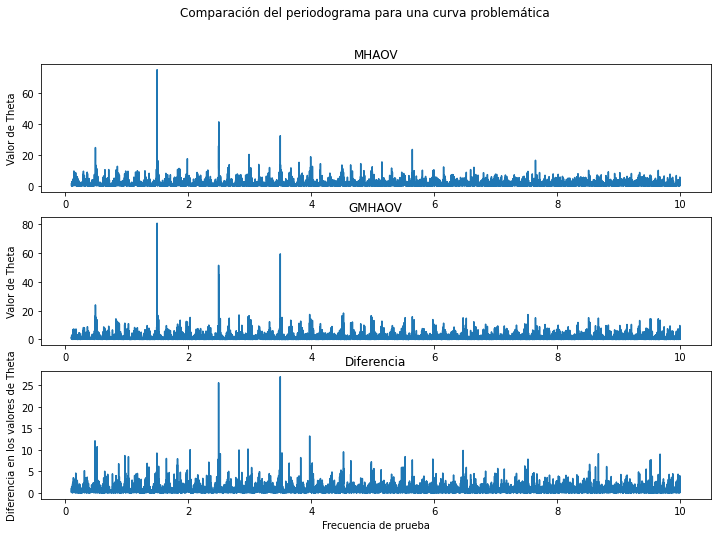
\includegraphics[width=0.8\textwidth]{figs/problemas.png}
    \caption{Resultado del periodograma para MHAOV (Arriba) y GMHAOV (Centro), y la diferencia entre ambos (Abajo).}
    \label{fig:problemas}
\end{figure}
En la figura \ref{fig:problemas} se pueden apreciar que la diferencia entre ambos periodogramas es notable, en especial en los peaks que están desplazados levemente, pero no es suficiente como para cambiar a las principales señales significativas, y de hecho al comparar la precisión de ambos algoritmos, esta solamente disminuye desde $80\%$ a $79\%$ para RR Lyrae.
\section{Efecto de el promediado de subarmónicos}\label{sec:efectos-subarmonicos}

Se evaluó el efecto en la precisión del GMHAOV y GCE al introducir el promediado de subarmónicos usando los conjuntos de datos mencionados en \ref{sec:mhaov-vs-gce}. 
\subsection{Promediado de subarmónicos}
\subsubsection{RR Lyrae}
En la tabla \ref{table:rrl-PS}, se observa que si bien PS logra obtener el periodo correcto para algunos objetos, los objetos para los que ya no se tiene el periodo correcto son casi el doble para ambos algoritmos. De la tabla \ref{table:rrl-PS-detalle} se puede notar que al aplicar PS en GCE, la cantidad de submúltiplos se reduce casi en un $50\%$, pero la cantidad de múltiplos casi se triplica, mientras que en GMHAOV los múltiplos incrementan levemente mientras que los submúltiplos se eliminan completamente.

\begin{table}[H]
\caption{Diferencias en la precisión de GCE y GMHAOV al aplicar promediado de subarmonicos (PS).}
\begin{tabular}{|c|c|c|c|c|}
\hline
Prueba & \begin{tabular}[c]{@{}c@{}}Ambos\\ aciertan\\ {[}\%{]}\end{tabular} & \begin{tabular}[c]{@{}c@{}}Acierta con\\ PS {[}\%{]}\end{tabular} & \begin{tabular}[c]{@{}c@{}}Deja de acertar\\ con PS {[}\%{]}\end{tabular} & \begin{tabular}[c]{@{}c@{}}No acierta\\ nunca {[}\%{]}\end{tabular} \\ \hline
GMHAOV & 90.15 & 0.10 & 0.20 & 9.55 \\ \hline
GCE & 52.10 & 3.70 & 6.70 & 37.50 \\ \hline
\end{tabular}
\label{table:rrl-PS}
\end{table}

\begin{table}[H]
\caption{Detalles de las diferencias en la precisión de GCE y GMHAOV al aplicar promediado de subarmonicos (PS).}
\begin{tabular}{|c|c|c|c|c|c|}
\hline
Prueba & Match & Multiplo & Submultiplo & Alias & Other \\ \hline
GMHAOV & 90.35 & 0.75 & 0.10 & 1.45 & 7.35 \\ \hline
\begin{tabular}[c]{@{}c@{}}GMHAOV\\ con PS\end{tabular} & 90.25 & 0.95 & 0.00 & 1.45 & 7.25 \\ \hline
GCE & 58.80 & 2.10 & 4.45 & 3.60 & 31.05 \\ \hline
\begin{tabular}[c]{@{}c@{}}GCE\\ con PS\end{tabular} & 55.80 & 5.90 & 2.45 & 4.05 & 31.80 \\ \hline
\end{tabular}
\label{table:rrl-PS-detalle}
\end{table}

\subsubsection{Binarias eclipsantes}
De las tablas \ref{table:eb-PS} y \ref{table:eb-PS-detalle}, se observa que en este caso no es beneficioso considerar el PS

\begin{table}[H]
\caption{Detalles de las diferencias en la precisión de GCE y GMHAOV al aplicar promediado de subarmonicos (PS) para binarias elipsantes.}
\begin{tabular}{|c|c|c|c|c|c|}
\hline
Prueba & Match & Multiplo & Submultiplo & Alias & Other \\ \hline
GMHAOV & 0.20 & 93.55 & 0.00 & 0.00 & 6.55 \\ \hline
\begin{tabular}[c]{@{}c@{}}GMHAOV\\ con PS\end{tabular} & 0.20 & 92.55 & 0.00 & 0.00 & 7.25 \\ \hline
GCE & 9.85 & 44.40 & 0.30 & 0.95 & 44.50 \\ \hline
\begin{tabular}[c]{@{}c@{}}GCE\\ con PS\end{tabular} & 7.75 & 45.56 & 0.10 & 0.80 & 45.85 \\ \hline
\end{tabular}
\label{table:eb-PS-detalle}
\end{table}
\begin{table}[H]
\caption{Diferencias en la precisión de GCE y GMHAOV al aplicar promediado de subarmonicos (PS) para binarias elipsantes.}
\begin{tabular}{|c|c|c|c|c|}
\hline
Prueba & \begin{tabular}[c]{@{}c@{}}Ambos\\ aciertan\\ {[}\%{]}\end{tabular} & \begin{tabular}[c]{@{}c@{}}Acierta con\\ PS {[}\%{]}\end{tabular} & \begin{tabular}[c]{@{}c@{}}Deja de acertar\\ con PS {[}\%{]}\end{tabular} & \begin{tabular}[c]{@{}c@{}}No acierta\\ nunca {[}\%{]}\end{tabular} \\ \hline
GMHAOV & 0.20 & 0.00 & 0.00 & 99.80 \\ \hline
GCE & 7.2 & 0.55 & 2.65 & 89.60 \\ \hline
\end{tabular}
\label{table:eb-PS}
\end{table}

\subsection{Efecto de el promediado de armónicos}\label{sec:efectos-subarmonicos}
Como se observó en algunos periodogramas, usualmente hay una señal significante en el doble de la frecuencia en vez de la mitad, así que se decide probar el promediado con la medida de confianza en el doble de la frecuencia, y le denominaremos a esto promediado de armónicos (PA).
\subsubsection{RR Lyrae}
De la tabla \ref{table:rrl-PA}, se reduce la cantidad de múltiplos como es de esperar, pero el efecto negativo del PA lleva a su efecto neto sea negativo.

\begin{table}[H]
\caption{Detalle de la precisión para GMHAOV y GCE al aplicar PA para RR Lyrae.}
\begin{tabular}{|c|c|c|c|c|c|}
\hline
Prueba & Match & Multiplo & Submultiplo & Alias & Other \\ \hline
GMHAOV & 90.35 & 0.75 & 0.1 & 1.45 & 7.35 \\ \hline
\begin{tabular}[c]{@{}c@{}}GMHAOV\\ con PA\end{tabular} & 90.40 & 0.25 & 0.20 & 1.75 & 7.40 \\ \hline
GCE & 58.80 & 2.10 & 4.45 & 3.60 & 31.05 \\ \hline
\begin{tabular}[c]{@{}c@{}}GCE\\ con PA\end{tabular} & 57.95 & 1.85 & 5.95 & 3.50 & 30.75 \\ \hline
\end{tabular}
\label{table:rrl-PA}
\end{table}

\subsubsection{Binarias Eclipsantes}
En el caso de las binarias eclipsantes, al aplicar PA la precisión incrementa más de 10 veces para GMHAOV y más de 3 veces para GCE. La cantidad de múltiplos se reduce significativamente, sin aumentar proporcionalmente la cantidad de submúltiplos.
\begin{table}[H]
\caption{Detalle de la precisión para GMHAOV y GCE al aplicar PA para binarias eclipsantes.}
\begin{tabular}{|c|c|c|c|c|c|}
\hline
Prueba & Match & Multiplo & Submultiplo & Alias & Other \\ \hline
GMHAOV & 0.20 & 93.25 & 0.00 & 0.00 & 6.55 \\ \hline
\begin{tabular}[c]{@{}c@{}}GMHAOV\\ con PA\end{tabular} & 3.30 & 89.96 & 0.00 & 0.20 & 6.90 \\ \hline
GCE & 9.85 & 44.40 & 0.30 & 0.95 & 44.50 \\ \hline
\begin{tabular}[c]{@{}c@{}}GCE\\ con PA\end{tabular} & 32.30 & 21.85 & 0.85 & 1.40 & 43.60 \\ \hline
\end{tabular}
\label{table:eb-PA}
\end{table}

\section{Comparación de rendimiento}\label{sec:rendimiento}
Para la evaluación del rendimiento, se usó el generador de curvas de luz incluido en el repositorio de MHAOV, que permite generar curvas de luz con ruido simulado y una determinada cantidad de puntos fácilmente. Se evaluó el rendimiento de MHAOV, GMHAOV, GCE y el impacto el promediado de subarmónicos en el tiempo de ejecución de GMHAOV para $N=10,\ldots,10^{4}$ curvas de luz con $150$ puntos cada una, el promedio para ALeRCE y una resolución de frecuencias de $\text{fres}=10^{-2}, 10^{-3}, 10^{-4}, 10^{-5}$ en un rango de $0.7$. MHAOV se lanza dividiendo las curvas en $8$ y ejecutandolo de forma paralela en CPU.

Para cada combinación de valores de prueba, se mide el tiempo de ejecución de MHAOV, GMHAOV, GCE y el promediado de subarmónicos, y los resultados se encuentran en la figura \ref{fig:benchmarks}. El tiempo de ejecución por curva se encuentra en la figura \ref{fig:benchmark-por-curva}
\begin{figure}[h]

    \centering
    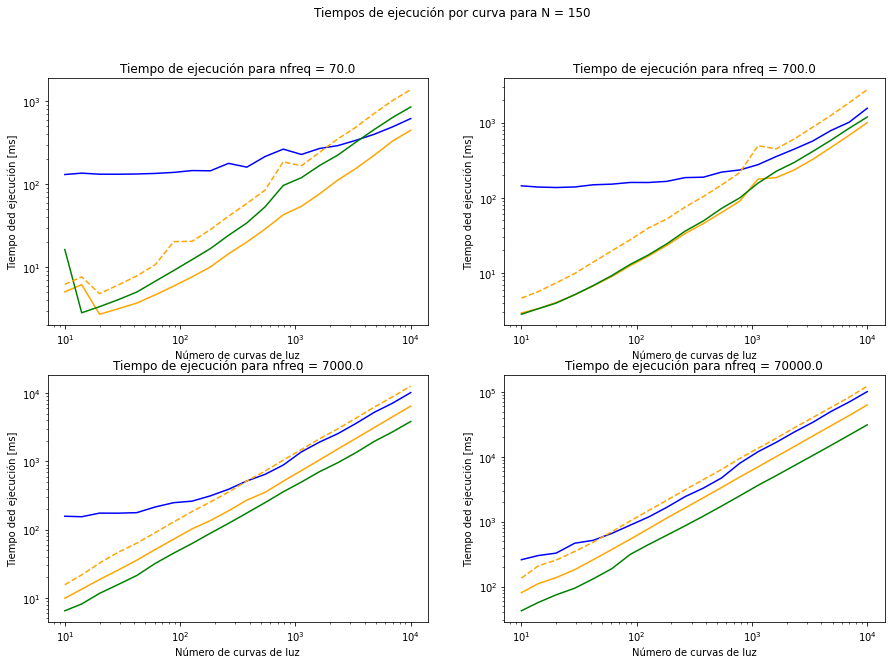
\includegraphics[width=0.8\textwidth]{figs/benchmarks-total.png}
    \caption{Resultados de las pruebas para cada combinación de frecuencias y número de curvas de luz simultaneas. La linea punteada representa el tiempo de ejecución de MHAOV sumado al tiempo de ejecución del promediado de subarmónicos.}
    \label{fig:benchmarks}
\end{figure}

\begin{figure}[h]
    \centering
    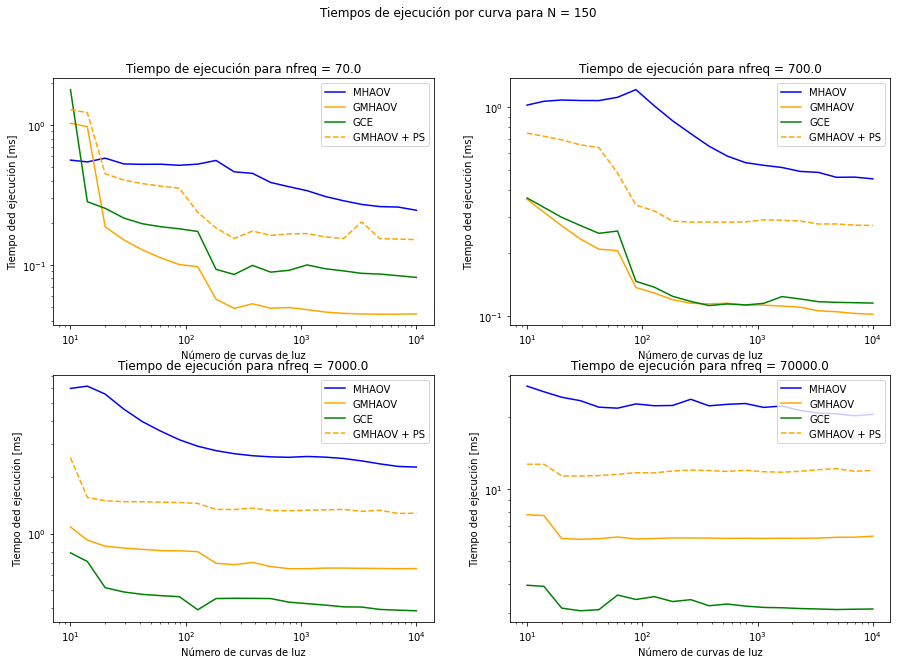
\includegraphics[width=0.8\textwidth]{figs/benchmarks.png}
    \caption{Tiempo de ejecución por curva para los algoritmos, incluyendo el tiempo de GMHAOV junto con el promediado de subarmónicos.}
    \label{fig:benchmark-por-curva}
\end{figure}

Incluso para resoluciones muy bajas de frecuencia, el tiempo de ejecución de los algoritmos paralelos es significativamente menor a $MHAOV$ para una cantidad de curvas menor a $10^{4}$, pero para resoluciones más cercanas a las usadas en la práctica, MHAOV nunca tiene un tiempo de ejecución mejor que GMHAOV y GCE, y GMHAOV se ejecuta más rápido que GCE. Sin embargo, si se le suma el tiempo de ejecución del promediado de subarmónicos, el tiempo de ejecución de GMHAOV es comparable al de su versión secuencial (ver Figura \ref{fig:benchmarks}).

Esta tendencia queda más clara con la figura \ref{fig:benchmark-per-curva}, donde para resoluciones de frecuencia más bajas el tiempo por curva de MHAOV llega a ser mejor que el de GCE, pero a medida que aumenta la resolución de frecuencia la eficiencia por curva de  MHAOV se hace cada vez menor que la de los algoritmos en GPU, con GMHAOV representando una mejora sustancial del tiempo de ejecución por curva.

Es importante destacar, sin embargo, que el tiempo de ejecución en GPU y del promediado de subarmónicos depende de la cantidad de curvas de una forma casi lineal, y tiene una dependencia más fuerte de la cantidad de frecuencias de prueba, como se observa en la figura \ref{fig:benchmark-frecuencias-prueba}. El tiempo de ejecución por curva por frecuencia de prueba de GCE disminuye con mayor rapidez que GMHAOV, lo que explica su mejor desempeño para una mayor resolución de frecuencias.

\begin{figure}[H]
    \centering
    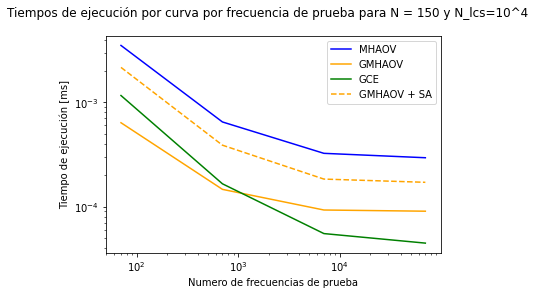
\includegraphics[width=0.8\textwidth]{figs/benchmarks-frequency.png}
    \caption{Variación del tiempo de ejecución por curva por frecuencia de prueba en función de la cantidad de frecuencia de pruebas para $N=10^{4}$}
    \label{fig:benchmark-frecuencias-prueba}
\end{figure}

\chapter{Análisis y conclusión}\label{chap:conclusión}
En este capitulo se hacen conclusiones a partir de los resultados, y se discute el trabajo futuro.
\section{Análisis de los resultados}\label{sec:analisis}
Es de gran importancia determinar que características de las curvas de luz problemáticas descritas en \ref{sec:validacion} causan la diferencia en los periodogramas obtenidos por MHAOV y su versión en GPU. Sin embargo, el efecto de esta diferencia, si bien es significativo, no cambia completamente los resultados del periodograma, al menos con los tipos de curvas con las que se hicieron pruebas.

De los resultados de la sección \ref{sec:efectos-subarmonicos}, se observa que considerar el PS o PA puede ser beneficioso en algunos casos, y se cree que si se le da el puntaje asociado a la frecuencia elegida por el periodograma al clasificador, este podrá aprender a discriminar en que situaciones es bueno considerar este puntaje y en cuales se puede ignorar. Además, por lo descrito en \ref{sec:rendimiento}, GMHAOV es una mejora tan significativa que si se incluye el cálculo de estos puntajes el tiempo de ejecución será menor al de MHAOV a menos que se procesen una cantidad de curvas del orden de $10^{4}$.

Además, de las pruebas de rendimiento se puede concluir que a pesar de que GCE es más rápido que GMHAOV, la precisión de MHAOV es mucho mejor por lo que la implementación de esta versión del algoritmo de calculo de periodos reduciría significativamente el tiempo de ejecución.

\section{Conclusión y trabajo futuro}\label{sec:conclusion}
En este trabajo se logró implementar un periodograma en GPU capaz de encontrar el periodo de una gran cantidad de curvas de luz de forma paralela, y además se estudio un posible algoritmo que puede identificar en algunos casos que el periodograma identifica una señal falsa como la frecuencia, por lo que el objetivo general fue cumplido. Sin embargo, por términos de tiempo no lograron cumplir los objetivos $4$ y $5$, pues no se pudo evaluar el impacto de usar los resultados de GMHAOV y GCE, y quizás los puntajes obtenidos usando PR y PA como características del clasificador de alerce. Es difícil predecir el impacto que tendrían la inclusión de estas estadísticas en el clasificador, ya que es un algoritmo de machine learning, pero si este algoritmo logra aprender cuando darle más peso a cada una de estas características, la mejora en la clasificación podría ser significativa para las clases relevantes.

A pesar de que el efecto de las imprecisiones en GMHAOV que no están presentes en su versión secuencial no sea severo, es importante identificar su causa pues puede serlo para objetos en los que no se realizaron pruebas y afectar severamente el clasificador. Si es que se logra encontrar la causa de los problemas mencionados, se debe llevar a cabo la implementación y testing de GMHAOV en el sistema de ALeRCE. Esto puede ser relativamente simple, ya que GMHAOV ofrece una interfaz en Python similar a la de MHAOV, pero se requeriría una validación más profunda del algoritmo.

Finalmente, debido a GMHAOV tiene un speedup significativo, estudiar el efecto del número de armónicos usados en el cálculo del periodograma tanto en su precisión como en su eficiencia puede solucionar el problema de la precisión sin un impacto muy grande en la eficiencia.

\bibliography{refs}
